\documentclass[11pt]{amsart}
%prepared in AMSLaTeX, under LaTeX2e
\addtolength{\oddsidemargin}{-.7in}
\addtolength{\evensidemargin}{-.7in}
\addtolength{\topmargin}{-.6in}
\addtolength{\textwidth}{1.5in}
\addtolength{\textheight}{1.3in}
\newcommand{\normalspacing}{\renewcommand{\baselinestretch}{1.05}
        \tiny\normalsize}

\newtheorem*{thm}{Theorem}
\newtheorem*{defn}{Definition}
\newtheorem*{example}{Example}
\newtheorem*{problem}{Problem}
\newtheorem*{remark}{Remark}

\usepackage{amssymb,fancyvrb,alltt,xspace}
\usepackage{hyperref}
\usepackage{palatino}
\usepackage{fancyvrb}


\usepackage[final]{graphicx}

\DefineVerbatimEnvironment{mVerb}{Verbatim}{numbersep=2mm,
frame=lines,framerule=0.1mm,framesep=2mm,xleftmargin=4mm,fontsize=\small}

% macros
\newcommand{\bb}{\mathbf{b}}
\newcommand{\bv}{\mathbf{v}}
\newcommand{\bx}{\mathbf{x}}
\newcommand{\by}{\mathbf{y}}

\newcommand{\CC}{\mathbb{C}}
\newcommand{\Div}{\nabla\cdot}
\newcommand{\eps}{\epsilon}
\newcommand{\grad}{\nabla}
\newcommand{\ZZ}{\mathbb{Z}}
\newcommand{\ip}[2]{\ensuremath{\left<#1,#2\right>}}
\newcommand{\lam}{\lambda}
\newcommand{\lap}{\triangle}
\newcommand{\RR}{\mathbb{R}}

\newcommand{\prob}[1]{\bigskip\noindent\large\textbf{#1}.\,\normalsize }
\newcommand{\ppart}[1]{\textbf{(#1)}\,\, }
\newcommand{\epart}[1]{\medskip\noindent\textbf{(#1)}\,\, }

%\newcommand{\pts}[1]{\scriptsize [#1 points] \normalsize}
\newcommand{\pts}[1]{}

\newcommand{\Matlab}{\textsc{Matlab}\xspace}
\newcommand{\Octave}{\textsc{Octave}\xspace}
\newcommand{\MO}{\Matlab/\Octave}


\begin{document}
\hfill \Large Name:\underline{\phantom{Ed Bueler really really long long long name}}
\medskip

\scriptsize \noindent Math 310 Numerical Analysis (Bueler) \hfill December 2019
\medskip

\Large\centerline{\textbf{SAMPLE Final Exam}}

\smallskip
\large
\begin{center}
\textbf{In class.  No book or electronics.  1/2 sheet of notes allowed.  120 minutes maximum.}
\end{center}

\bigskip
\thispagestyle{empty}
\normalspacing

\prob{1} \pts{10} Write a \Matlab code for the Newton method applied to the problem $f(x)=0$:

\centerline{\texttt{function x = newton(f,dfdx,x0)}}

\noindent The inputs are $f=$ \texttt{f}, the derivative $f'=$ \texttt{dfdx}, and an initial estimate $x_0=$ \texttt{x0}.  Stop the algorithm (\emph{show this in the code!}) when $|f(x)| \le 10^{-6}$.
\vfill


\prob{2} \ppart{a} \pts{10} State the polynomial interpolation error theorem (with a remainder term).  \emph{Carefully state the hypotheses \emph{and} the conclusion of the theorem.}
\vspace{2.0in}

\epart{b} \pts{5}  Assume the interval in question is $[-1,1]$ and that the interpolation points are the Chebyshev points $x_j = \cos(\pi j/n)$ for $n=0,1,2,\dots,n$.  What can you say about the remainder term that explains why the Chebyshev points are effective for interpolation?  \emph{Answer in a couple of complete sentences.}
\vspace{1.0in}


\newpage
\prob{3} \ppart{a} \pts{10}   Consider
  $$f(x) = \frac{1}{x+2}.$$
Completely set up, but do not solve, the Vandermonde system to find the degree 3 polynomial $p(x)$ which interpolates $f(x)$ at the points $x_0=-1.5,x_1=-1,x_2=0,x_3=1$.
\vfill

\epart{b} \pts{10}  For the same $f(x)$ and interpolation points as in part \textbf{(a)}, write down Lagrange's form of the polynomial $p(x)$.   Do not simplify.
\vfill

\prob{4}  \pts{10}   Table 10.3 includes the error formula for Simpson's rule: if $f \in C^4[a,b]$ then
	$$\int_a^b f(x)\,dx = \frac{b-a}{6} \left[f(a) + 4 f\left(\frac{a+b}{2}\right) + f(b)\right] + \frac{1}{2880} (b-a)^5 f^{(4)}(\xi)$$
for some $\xi \in [a,b]$.  Why does this fact show that Simpson's rule is exact if $f(x)$ is a cubic polynomial?  \emph{Answer in at least one complete sentence.}
\vfill


\newpage
\prob{5}  \ppart{a} \pts{10}  Find $A_0$ and $A_1$ so that the numerical integration rule
	$$\int_{-1}^1 f(x)\,dx \approx A_0 f(-\tfrac{1}{2}) + A_1 f(+\tfrac{1}{2})$$
is exact for all degree at most one polynomials.  (I.e.~for all linear functions.)
\vfill

\epart{b} \pts{10} Show that the rule generated in part \textbf{(a)} is \emph{not} exact for degree two polynomials.
\vfill

\prob{6}  \pts{10}  Recall that if $\ell(x)$ is the piecewise-linear interpolant of $f \in C^2[a,b]$ at equally-spaced points $x_0=a<x_1<x_2<\dots<x_n=b$, with spacing $h=(b-a)/n$, then
	$$|f(x) - \ell(x)| \le \frac{Mh^2}{8}$$
for all $x\in[a,b]$, where $M=\max_{x\in[a,b]}|f''(x)|$.  Find $n$ so that the error is at most $2 \times 10^{-4}$ in using such equally-spaced linear interpolation for $f(x)=e^{-x}$ on $[a,b]=[0,2]$.
\vfill


\newpage
\prob{7} \pts{10}  Do two steps of the Euler method, with step size $h=1$, on the ODE IVP
	$$y' = t - y, \qquad y(0)=1.$$
\vfill

\prob{8} \ppart{a} \pts{10}  Sketch one step of the midpoint method for the general ODE IVP
	$$y' = f(t,y), \qquad y(t_0)=y_0$$
where $t_{k+1}-t_k = h$ is the step size.
(Hints:  \emph{Your sketch will have $t$ and $y$ axes.  Show the current iterate $(t_k,y_k)$ and all the locations where a slope is computed.  Show how to compute the new iterate $y_{k+1}$.})
\vfill

\epart{b} \pts{3}  Show that the midpoint method is exact when solving the ODE IVP
	$$y' = 2 t - 8, \qquad y(2)=3.$$
\vspace{1.5in}


\newpage
\prob{9} \pts{10}  Suppose the IEEE 754 standard for floating point representations had a 9 bit version:

\medskip\large
\begin{center}
\begin{tabular}{|c|c|c|c|c|c|c|c|c|} \hline
$s$ & $e_1$ & $e_2$ & $e_3$ & $b_1$ & $b_2$ & $b_3$ & $b_4$ & $b_5$ \\ \hline
\end{tabular}
\end{center}
\medskip\normalsize

\noindent representing the number
\medskip\large
	$$x = (-1)^s\,(1.b_1 b_2 b_3 b_4 b_5)_2 \,\, 2^{(e_1 e_2 e_3)_2 - 3_{10}}$$
\normalsize

\noindent Note the exception cases:
\begin{itemize}
\item exponent bits $(000)_2$ define the number zero or subnormal numbers
\item exponent bits $(111)_2$ define the other exceptions: $\pm\infty$ and NaN (\emph{\dots ignore the details})
\end{itemize}

\epart{a}  What is the largest real number that this system can represent?  (\emph{State the number in decimal notation and show the bits.})
\vspace{1.2in}

\epart{b}  What is the value of ``machine epsilon'' in this system?  (\emph{State the number in decimal notation.})
\vspace{1.2in}

\prob{10} \pts{10}  Suppose we want to use Taylor's theorem to compute values of $\sin x$ for $|x|<0.5$ to an accuracy of $10^{-3}$.  Use the Taylor theorem with remainder to determine how many terms, i.e.~what $n$, is needed to do this.
\vfill

\newpage
\prob{11}  \pts{10}  Solve the following system of linear equations by Gauss elimination with partial pivoting and back substitution.  Show your steps.
\begin{align*}
2 x_1 + 2 x_2 &= 6 \\
4 x_1 - 3 x_2 &= -2.
\end{align*}
\vfill

\prob{12} \pts{10}  The high-level view of the Gauss elimination with partial pivoting algorithm is that, given a linear system 
  $$A \bx = \bb,$$
it computes matrices $P,L,U$ so that $PA=LU$.  What properties do these matrices have?  (\emph{Write at least two complete sentences.})  Then explain how to solve the linear system, indicating how much work is required at each stage.  (\emph{Write at least two complete sentences.})
\vfill

\newpage
\prob{13} \ppart{a} \pts{10}  Write a \Matlab algorithm for multiplying a square $n\times n$ matrix $A$ by an $n\times 1$ column vector $\mathbf{v}$.  In particular, fill in the rest of the function below to compute
  $$\mathbf{z} = A \mathbf{v}.$$
I have written the first line to get $n$.  You may assume all sizes of the inputs are correct; there is no need to check these sizes.  Do not use matrix-vector multiplication inside this routine; pretend that we are writing this for the first time and use \texttt{for} loops.
\begin{mVerb}
function z = mattimesvec(A,v)
% MATTIMESVEC multiplies A by v and gives z

n = length(v);
























\end{mVerb}

%function z = mattimesvec(A,v)
%% MATTIMESVEC multiplies A by v and gives z
%
%n = length(v);
%z = zeros(size(v));
%for i = 1:n
%  z(i) = A(i,1) * v(1);
%  for j = 2:n
%    z(i) = z(i) + A(i,j) * v(j);
%  end
%end

\epart{b} \pts{5}  Count the floating point operations in the above algorithm.
\vspace{2.0in}


%\epart{c} \pts{5}  Is the number of operations in the part \textbf{(a)} algorithm more or less than the number of operations needed to do Gauss elimination on a system of $n$ linear equations in $n$ unknowns?
%\vfill


\newpage
\begin{center}
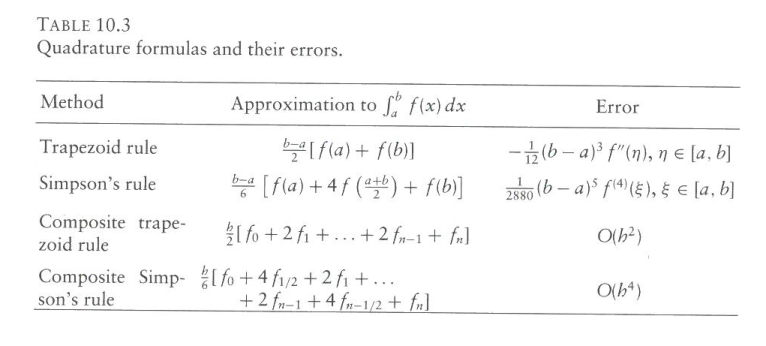
\includegraphics[width=0.95\textwidth]{figs/inttable}
\bigskip

%\noindent \hrulefill

[BLANK SPACE FOR SCRATCH WORK]
\end{center}
\thispagestyle{empty}
\vfill

\end{document}
